%%%%%%%%%%%%%%%%%%%%%%%%%%%%%%%%%%%%%%%%%%%%%%%%%%%%%%%%%%%%%%%%%%%%%%
% LaTeX Template: Project Titlepage
%
% Source: http://www.howtotex.com
% Date: April 2011
% 
% This is a title page template which be used for articles & reports.
% 
% Feel free to distribute this example, but please keep the referral
% to howtotex.com
% 
%%%%%%%%%%%%%%%%%%%%%%%%%%%%%%%%%%%%%%%%%%%%%%%%%%%%%%%%%%%%%%%%%%%%%%
% How to use writeLaTeX: 
%
% You edit the source code here on the left, and the preview on the
% right shows you the result within a few seconds.
%
% Bookmark this page and share the URL with your co-authors. They can
% edit at the same time!
%
% You can upload figures, bibliographies, custom classes and
% styles using the files menu.
%
% If you're new to LaTeX, the wikibook is a great place to start:
% http://en.wikibooks.org/wiki/LaTeX
%
%%%%%%%%%%%%%%%%%%%%%%%%%%%%%%%%%%%%%%%%%%%%%%%%%%%%%%%%%%%%%%%%%%%%%%
%
% --------------------------------------------------------------------
% Preamble
% --------------------------------------------------------------------
\documentclass[paper=a4, fontsize=11pt,twoside]{scrartcl}	% KOMA

\usepackage[a4paper,pdftex]{geometry}	% A4paper margins
\setlength{\oddsidemargin}{5mm}			% Remove 'twosided' indentation
\setlength{\evensidemargin}{5mm}

\usepackage[english]{babel}
\usepackage[protrusion=true,expansion=true]{microtype}	
\usepackage{amsmath,amsfonts,amsthm,amssymb}
\usepackage{graphicx}
\usepackage{float}
\usepackage{algorithm}
\usepackage[noend]{algpseudocode}
\usepackage{wrapfig}
% --------------------------------------------------------------------
% Definitions (do not change this)
% --------------------------------------------------------------------
\newcommand{\HRule}[1]{\rule{\linewidth}{#1}} 	% Horizontal rule

\makeatletter							% Title
\def\printtitle{%						
    {\centering \@title\par}}
\makeatother									

\makeatletter							% Author
\def\printauthor{%					
    {\centering \large \@author}}				
\makeatother							

% --------------------------------------------------------------------
% Metadata (Change this)
% --------------------------------------------------------------------
\title{	\normalsize \textsc{Project Report} 	% Subtitle
		 	\\[2.0cm]								% 2cm spacing
			\HRule{0.5pt} \\						% Upper rule
			\LARGE \textbf{\uppercase{Sample Sizes for Query Probing in Distributed Information Retreival}}	% Title
			\HRule{2pt} \\ [0.5cm]		% Lower rule + 0.5cm spacing
			\normalsize \today			% Todays date
		}

\author{
		Rahul Ramakrishna\\	
		University of Massachussets Amherst\\	
		Dept Of Computer Science\\
        \texttt{rahulram@cs.umass.edu} \\
}


\begin{document}
% ------------------------------------------------------------------------------
% Maketitle
% ------------------------------------------------------------------------------
\thispagestyle{empty}		% Remove page numbering on this page

\printtitle					% Print the title data as defined above
  	\vfill
\printauthor				% Print the author data as defined above
\newpage
% ------------------------------------------------------------------------------
% Begin document
% ------------------------------------------------------------------------------
\setcounter{page}{1}		% Set page numbering to begin on this page
\section{Introduction}

In Distributed Information Reterival systems, information is held in separate collections, which might be in different physical locations or on separate servers. The query is first passed to a central
broker. The broker then sends this query to all or some of the servers. The cost of networking during query execution seems an overhead, escepially if the query is sent to servers which dont have similar collections.

\begin{figure}[H]
\centering
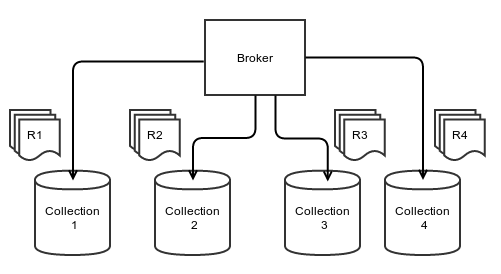
\includegraphics[width=\textwidth]{./img/ir.png}
\caption{\label{fig:1}DIR System.}
\end{figure}


Thus, DIR has 2 major issues to be resolved. 
\begin{enumerate}
\item Selection of a particular collection
\item Merging of Results.
\end{enumerate}
In this report, we are mainly focusing on selection of collections. We are focusing on how to characterize a 
particular collection such that, the broker can decide on which servers to send the queries to further probe for 
results. We further explore 2 main sampling techniques which are used to represent collection of sets.


\makeatletter
\def\BState{\State\hskip-\ALG@thistlm}
\makeatother

\section{Query Probing}
In non-cooperative environments like distributed systems. We dont get index information from each of the collections that are being fetched. Instead, its the brokers that constantly probe into the collection by sending artificial queries in random order and evaluate returned answers. The answers are called \texttt{probes} 
and the process is called \texttt{query probing}. For example, if we send a series of single probe queries such as "books", "football", "ibm" and the following number of answers are returned: 1000, 200, 450 . From the results we can guess that, the documents are more likely to talk about Books and IBM rather than football. 


The following is the algorithm initially proposed by Callan et al [1], which iteratively discovers the 
language model of the collections in non-cooperative environments.The language model is updated 
according to the new terms found in the retrieved documents. The next probe queries are selected from the obtained language model. Probing continues until a stopping criterion is met.




\begin{algorithm}
\caption{Query Sampling}\label{Query Sampling}
\begin{algorithmic}[1]
\Procedure{QS}{}
\State Select an Initial Query Term
\State Run Query on the IR System
\State Reterive Top N Documents as Result.
\State Update the Resource Description based on characterstics of retreived documents. 
\BState \emph{loop}:
\State for words,freq in Documents
\State Update Learned Resource Descriptions.

\If {$\textit{StopCriteria()} = \textit{Yes}$}
\State break;
\Else 
\State Goto 3
\EndIf
\EndProcedure
\end{algorithmic}
\end{algorithm}



Callan et al suggested that assigning $N = 4$  and  $StopCriteria = 75$ Docs i.e examining a total of 300 documents will be a good representation of the collection. The algorithm has many open ended choices which needs to be tuned. For example, how to select query terms and how to select documents to examin per query and most importantly \textit{when to stop sampling}. In the subsequent sections we will evaluate sampling techniques mentioned by Callan et al and adaptive query probing techniques by Milad et al [2]. 


\section{Sampling Techniques}
\label{sec:examples}


\subsection{Static Sampling using Ctf}

In static sampling technique. The paper uses a Character term frequency as a metric in order to calibrate the sample size. \textit{Ctf} ratio is defined as the ratio of  term occurences in the collection that are covered by terms in the learned resource description. For the learned vocublary $V'$ and actual vocabulary $V$, 

$$Ctf = \frac{\sum_{i\epsilon V'}  ctf_i}{\sum_{i\epsilon V} ctf_i}$$

$ctf_i$ is the number of times the term i occurs in the database (collection term frequency or \textit{ctf}).
The \textit{ctf} ratio is computed after the stopwords were removed. 
Experiments performed by Callan et al suggested that the \textit{Ctf} curve usually smoothens at sample of 300 documents. Thus, making a general stopping criteria in query probing algorithms.


%Use \texttt{section}s and \texttt{subsection}s to organize your document. \LaTeX{} handles all the formatting and numbering automatically. Use \texttt{ref} and \texttt{label} for cross-references --- this is Section~\ref{sec:examples}, for example.


\subsection{Adaptive Query Probing}

In adaptive query technique, we extract the most significant terms from each collection by gathering all terms.
Cosine $tf.idf \geq \gamma $  Where $(\gamma)$ is a threshold value using Indrie. This information is used after termination of query-based sampling, as a measure of the effectiveness of the collected summaries and of the risk of missing significant terms.

\[ Term = \left\{ 
  \begin{array}{l l}
    Significant & \quad \text{if $tf.idf \geq \gamma$}\\
    \textit{Not Significant} & \quad \text{otherwise}
  \end{array} \right.\]



Queries from the Robust.qrels were choosen randomly. mostly, queries of size 2 - 4 terms were choosen, which were similar to web queries  [Jansen et al., 2000] . In this technique we make an assumption that collections only return a limited number of documents for any given query.

The Recall metric to measure completeness of a term set is defined as,

$$Recall(s,\gamma) = \frac{\text{No of Significant terms in sample}}{\text{Total No of Significant terms}}$$

we gather samples of different sizes ranging from 100 to 4000 documents to iteratively probe into them. In the further sections its explained that the the representation size of 4000 documents would meet the stopping criteria. 



% Commands to include a figure:
%\begin{figure}
%\includegraphics[width=\textwidth]{your-figure's-file-name}
%\caption{\label{fig:your-figure}Caption goes here.}
%\end{figure}

%\subsection{Mathematics}
%
%\LaTeX{} is great at typesetting mathematics. Let $X_1, X_2, \ldots, X_n$ be a sequence of independent and identically distributed random variables with $\text{E}[X_i] = \mu$ and $\text{Var}[X_i] = \sigma^2 < \infty$, and let
%$$S_n = \frac{X_1 + X_2 + \cdots + X_n}{n}
%      = \frac{1}{n}\sum_{i}^{n} X_i$$
%denote their mean. Then as $n$ approaches infinity, the random variables $\sqrt{n}(S_n - \mu)$ converge indistribution to a normal $\mathcal{N}(0, \sigma^2)$.

\section{Measure of Effectiveness}

All the experiments were performed on Robust dataset. We intend to verify the following hypothesis
\begin{enumerate}
\itemsep -0.5em
\item As long as we keep sampling, the vocabulary continues to grow.
\item The rate of vocabulary growth is not a good way to estimate collection size.
\item The risk of missing significant terms is high with traditional sampling.
\end{enumerate}



%You can make lists with automatic numbering \dots

\subsection{Ctf Ratios}
Using the static sampling algorithm proposed by Callan et all. The Ctf metric is been calculated for the robust dataset. The fig 2 shows the ctf ratio for the sample sizes ranging from $100$ to $2500$ sampled documents. 

\begin{figure}[H]
\centering
\includegraphics[width=\textwidth]{./img/ctf.png}
\caption{\label{fig:2}Ctf Ratio of Robust Collection.}
\end{figure}

The expected value of curve smoothing should be from 300. But as we can see from the graph, the smoothening of the curve begins from 500 documents. Thus, if probing is halted after sampling 300 documents,
the risk of losing significant terms is high. However, this value could be different for different collections, which makes it even more difficult validate \textit{Ctf} as a meteric to sample documents.

\subsection{Significant terms}

For calibrating siginificant terms, samples ranging from $100$ to $4000$ we extracted. Each sample $n$ contains all the documents from sample $n$ - $1$, plus 100 new documents. The initial sample always extracts 100 distinct documents. At any given point, the system calculates the number of unique and significant terms
available in the samples. We show results for $4000$ documents.

\begin{figure}[H]
\centering
\includegraphics[width=\textwidth]{./img/exp.png}
\caption{\label{fig:3}Statistics of Robust Collection.}
\end{figure}

From the fig 3 we can see that a sample of $4000$ documents would suffice for experiment testbed. Since, after $4000$, even though the vocabulary keeps growing, the addition of significant terms smoothens out. 
Convergence point , slope of the graph
For $\eta$  subsequent samples the rate of growth in vocabulary becomes less than threshold $\tau$ .


\subsection{Result Evaluation}

Retreived Documents 


\begin{figure}[H]
\centering
\includegraphics[width=\textwidth]{./img/relret.png}
\caption{\label{fig:3}Statistics of Robust Collection.}
\end{figure}

%\begin{wrapfigure}{L}{0.7\textwidth}
%\centering
%\includegraphics[width=0.70\textwidth]{./img/relret.png}
%\caption{\label{fig:frog2}This is a figure caption.}
%\end{wrapfigure}


MAP, P@10, P@20


\section{Conclusion}
Adaptive Query probing is a better way for summarizing collections in Distributed Information Retreival. Static sampling sizes using ctf ratio leads to considerable loss of effectiveness. Adaptive query has a better strategy of knowing, when to stop query probing. From the results we can see that, rate of arrival of new terms has
become constant, relatively few new significant terms of high impact in retrieval are observed.



\section{References}

\begin{enumerate}
  \item Query Based Sampling of Text Databases. Jamie Callan, Margaret Connell 
  \item Sample Sizes for Query Probing in Uncooperative Distributed Information Retrieval. Milad Shokouhi, 
  Falk Scholer, and Justin Zobel. 
\end{enumerate}

% ------------------------------------------------------------------------------
% End document
% ------------------------------------------------------------------------------
\end{document}
